% Figure 1
\ffigbox[\FBwidth]{
\caption{\centering Graphe \(G\)}\label{Fig:td1ex3c3}
}{
    \fbox{
        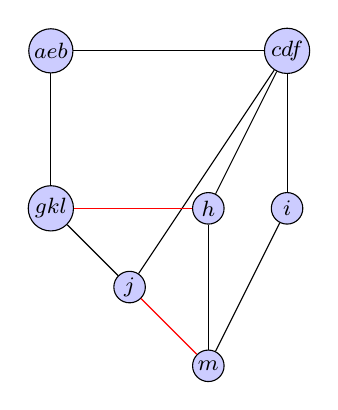
\begin{tikzpicture}[scale=1, every node/.style={circle, draw, fill=blue!20, inner sep=1pt, font=\footnotesize, minimum size=4mm}]
            \node (aeb) at (0, 2) {\(aeb\)};
            \node (cdf) at (3, 2) {\(cdf\)};
            \node (gkl) at (0, 0) {\(gkl\)};
            \node (h) at (2, 0) {\(h\)};
            \node (i) at (3, 0) {\(i\)};
            \node (j) at (1, -1) {\(j\)};
            \node (m) at (2, -2) {\(m\)};
            
            \draw (aeb) -- (gkl);
            \draw (aeb) -- (cdf);

            \draw (cdf) -- (j);
            \draw (cdf) -- (i);

            \draw (gkl) -- (j);
            \draw[red] (gkl) -- (h);

            \draw[red] (j) -- (m);
            
            \draw (i) -- (m);

            \draw (cdf) -- (h);

            \draw (h) -- (m);
        \end{tikzpicture}
    }
}